\documentclass[a4paper,11pt,titlepage]{article}
\usepackage{graphicx}
\author{Abrie Greeff\\B.Sc Hons (Computer Science)\\Department of Computer Science\\University of Stellenbosch}
\title{Data Encryption Using $\oplus$-NFAs}
\begin{document}
\maketitle
\tableofcontents
\section{Introduction}
Protecting information is of high importance for governments and corporations. The best method for protecting digital information is by using data encryption.
There are two different types of encryption, public key and private key encryption. When data is encrypted a key is used so that the data can be decrypted later. With private key encryption the key is only known to the persons who has access to this data. Public key encryption uses two different keys, one publicly available for encryption and one private key used for decryption.

There are two ways in which data can be processed when encrypting, it can be processed as blocks of characters called a block cipher or a stream of bits called a stream cipher.
This article will focus on implementing symmetric nondeterministic finite automata ($\oplus$-NFAs) as a private key block cipher system as discussed in [1].
\section {Constructing a cipher from a $\oplus$-NFA}
A NFA needs to be constructed that has the same amount of states as the amount of bits needed to represent one character. Computers use eight bits to represent unicode characters, therefore the NFA needs to have eight states. The success of the NFA depends on the transition function that is chosen to move between states.

An example of such a transition function is,\\
$\delta(q_i,a)=\overline{\{q_i,q_{i+1}\}}$, for $0\leq i \leq n-2$ and\\
$\delta(q_{n-1},a)=\overline{\{q_{n-1}\}}$


where \emph{n} is the number of states and \emph{$q_i$} is the current state. The transition table, for a 3-bit example, then looks as follows,

\begin{tabular}{|r|l|}
$\delta$ & a\\
\hline
0 & 01\\
1 & 12\\
2 & 2
\end{tabular}
\newline\\
The next step is to construct a deterministic finite automata (DFA) from this NFA using subset construction. The subset construction is done differently than is done normally by using an exclusive-not-or (XNOR) binary operation. This is done by first numbering all possible states of the DFA. These are the different permutations of bits that can occur. This gives $2^n$ possible states, where \emph{n} is the amount of states of the NFA.

For every state in the DFA the bits are checked and all the states corresponding to bits that are set are XNORed with each other. The DFA constructed from the NFA from the previous example then has the following transition table.
\newline\\
\begin{tabular}{|r|l|}
$\delta$ & a\\
\hline
0 & 7\\
1 & 6\\
2 & 4\\
3 & 5\\
4 & 1\\
5 & 0\\
6 & 2\\
7 & 3\\
\end{tabular}
\newline\\

This DFA has two looping cycles as seen in fig.1

\begin{figure}[htbp]
   \centering
   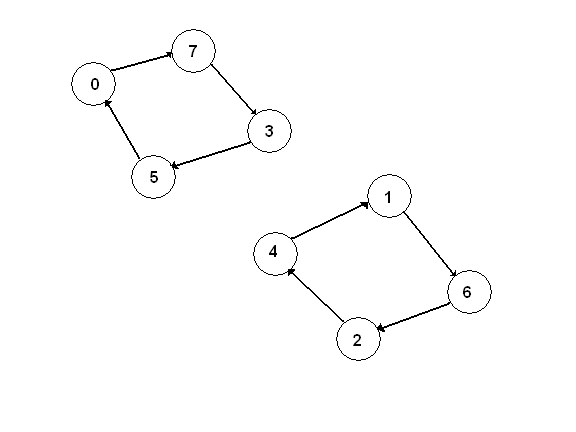
\includegraphics[width=7cm]{cycles.png}
   \caption{Cycles for 3-bit example}
   \label{Figure:figex}
\end{figure}

For the encryption to work it is important that these cycles contain the same amount of states and that the amount of states in each cycle are even. If these requirements are fulfilled the DFA can now be used to encrypt data. Encryption is done by reading a character, converting the character to its unicode value and then finding the state corresponding to this value in the transition table. Once this state has been found the NFA is traversed half of the cycle length. The state that has been reached now is the encrypted value of the original value. To decrypt this value the cycle is completed thus returning to the original value. To encrypt the data even more the value can be passed through a series of different DFAs thus decreasing the possibility of the data being compromised.
\section{Implementation}
The encryption algorithm was developed in Java. The program accepted a set of rules and a file name as parameters. The rules were defined as \emph{-ra:b}, where \emph{a} and \emph{b} are numbers that define the offsets from the current state to the states that needs to be XNORed when creating the NFA. More than one rule can be defined in the parameters as set out in Section 2. An array of eight values was used to store the NFA states because this is the the fastest and most efficient way it can be implemented. The DFA was stored in exactly the same way but was an array of 256 values to accommodate all the possible states. The DFA was created exactly as outlined in Section 2. After the DFA was created the cycles was counted and checked if they all satisfied the requirements. All the rules and half cycle lengths was then stored in another two arrays that were the size of the amount of rules.

When all the DFAs were created the encryption or decryption of the specified file started. The file was read one character at a time, encrypted or decrypted and then written to an output file.
\section{Testing}
The testing of the program was first done using different input files and one rule to see if two files were the same after encrypting the first one and the decrypting it again. After these tests were done another rule was added and the tests were repeated. I found that some rules gave incorrect cycles and was thus rejected as it should be. When the rules were all correct the program provided correct results and good encryption. When I tried to break the encryption it was not difficult because of the limited amount of good rules that are accepted by program and a brute force attack showed this problem.
\section{Conclusion}
This method gave good encrypted data because it behaves almost the same as a permutation cipher and permutation ciphers provide some of the best encryption that can be obtained from a block cipher. If the amount of bits that was used to do encrypt were changed it could have been possible to easily change the program into a stream cipher. The time complexity of the algorithm was very efficient and gives this method very good overall performance. This can be used as a low cost alternative to some algorithms that are available today. The only problem is that if someone knows this system was used it will be very easy to break the code because of the small amount of rules that satisfy the requirements.
\section{References}
\begin{enumerate}
\item Dr. L Van Zijl
\emph{$\oplus$-NFAs as Block Cipher Systems}, CS778:Course notes.
\end{enumerate}
\end{document}
